% ============================================================================
% 3Alternative-6-LogNormal.tex
% Model 6: Log-Normal GLM with Duan's Smearing Estimator
% Following the EXACT pattern from Models 1, 2, and 3
% NO UNICODE - All special characters in LaTeX math mode
% ============================================================================

\chapter{Model 6: Log-Normal GLM with Conditional Smearing}\label{ch:model6}

% Load model-specific values
% Model 6 Actual Values
% Generated: 2025-10-15 02:33:29

\renewcommand{\ModelSixRSquaredTrain}{-0.3626}
\renewcommand{\ModelSixRSquaredTest}{-0.3517}
\renewcommand{\ModelSixRMSETrain}{52,479.30}
\renewcommand{\ModelSixRMSETest}{51,923.33}
\renewcommand{\ModelSixRMSETrainSqrt}{1.22}
\renewcommand{\ModelSixRMSETestSqrt}{1.23}
\renewcommand{\ModelSixMAETrain}{35,825.09}
\renewcommand{\ModelSixMAETest}{35,373.73}
\renewcommand{\ModelSixMAPETrain}{405.14}
\renewcommand{\ModelSixMAPETest}{423.85}
\renewcommand{\ModelSixCVMean}{-0.3704}
\renewcommand{\ModelSixCVStd}{0.0754}
\renewcommand{\ModelSixCVCILower}{-0.5181}
\renewcommand{\ModelSixCVCIUpper}{-0.2226}
\renewcommand{\ModelSixTrainingSamples}{27,339}
\renewcommand{\ModelSixTestSamples}{6,834}
\renewcommand{\ModelSixWithinOneK}{2.49}
\renewcommand{\ModelSixWithinTwoK}{4.74}
\renewcommand{\ModelSixWithinFiveK}{14.27}
\renewcommand{\ModelSixWithinTenK}{26.84}
\renewcommand{\ModelSixWithinTwentyK}{48.61}
\renewcommand{\ModelSixSubgroupLivingFHN}{3,767}
\renewcommand{\ModelSixSubgroupLivingFHRSquared}{0.1024}
\renewcommand{\ModelSixSubgroupLivingFHRMSE}{30,173.35}
\renewcommand{\ModelSixSubgroupLivingFHBias}{-5,118.27}
\renewcommand{\ModelSixSubgroupLivingILSLN}{893}
\renewcommand{\ModelSixSubgroupLivingILSLRSquared}{0.2458}
\renewcommand{\ModelSixSubgroupLivingILSLRMSE}{35,010.45}
\renewcommand{\ModelSixSubgroupLivingILSLBias}{7,974.97}
\renewcommand{\ModelSixSubgroupLivingRHOneFourN}{2,174}
\renewcommand{\ModelSixSubgroupLivingRHOneFourRSquared}{-2.7981}
\renewcommand{\ModelSixSubgroupLivingRHOneFourRMSE}{79,962.36}
\renewcommand{\ModelSixSubgroupLivingRHOneFourBias}{57,051.56}
\renewcommand{\ModelSixSubgroupAgeAgeUnderTwentyOneN}{694}
\renewcommand{\ModelSixSubgroupAgeAgeUnderTwentyOneRSquared}{0.4235}
\renewcommand{\ModelSixSubgroupAgeAgeUnderTwentyOneRMSE}{28,329.45}
\renewcommand{\ModelSixSubgroupAgeAgeUnderTwentyOneBias}{-7,464.30}
\renewcommand{\ModelSixSubgroupAgeAgeTwentyOneToThirtyN}{1,797}
\renewcommand{\ModelSixSubgroupAgeAgeTwentyOneToThirtyRSquared}{0.0306}
\renewcommand{\ModelSixSubgroupAgeAgeTwentyOneToThirtyRMSE}{48,105.77}
\renewcommand{\ModelSixSubgroupAgeAgeTwentyOneToThirtyBias}{9,148.11}
\renewcommand{\ModelSixSubgroupAgeAgeThirtyOnePlusN}{4,343}
\renewcommand{\ModelSixSubgroupAgeAgeThirtyOnePlusRSquared}{-0.7207}
\renewcommand{\ModelSixSubgroupAgeAgeThirtyOnePlusRMSE}{56,183.71}
\renewcommand{\ModelSixSubgroupAgeAgeThirtyOnePlusBias}{23,166.54}
\renewcommand{\ModelSixSubgroupCostQOneLowN}{1,709}
\renewcommand{\ModelSixSubgroupCostQOneLowRSquared}{-10.0000}
\renewcommand{\ModelSixSubgroupCostQOneLowRMSE}{26,817.02}
\renewcommand{\ModelSixSubgroupCostQOneLowBias}{18,283.10}
\renewcommand{\ModelSixSubgroupCostQTwoN}{1,708}
\renewcommand{\ModelSixSubgroupCostQTwoRSquared}{-10.0000}
\renewcommand{\ModelSixSubgroupCostQTwoRMSE}{28,282.79}
\renewcommand{\ModelSixSubgroupCostQTwoBias}{11,028.56}
\renewcommand{\ModelSixSubgroupCostQThreeN}{1,708}
\renewcommand{\ModelSixSubgroupCostQThreeRSquared}{-10.0000}
\renewcommand{\ModelSixSubgroupCostQThreeRMSE}{53,516.01}
\renewcommand{\ModelSixSubgroupCostQThreeBias}{16,201.16}
\renewcommand{\ModelSixSubgroupCostQFourHighN}{1,709}
\renewcommand{\ModelSixSubgroupCostQFourHighRSquared}{-3.9867}
\renewcommand{\ModelSixSubgroupCostQFourHighRMSE}{80,000.53}
\renewcommand{\ModelSixSubgroupCostQFourHighBias}{19,963.16}
\renewcommand{\ModelSixCVActual}{1.0101}
\renewcommand{\ModelSixCVPredicted}{1.0513}
\renewcommand{\ModelSixPredictionInterval}{96,579.71}
\renewcommand{\ModelSixBudgetActualCorr}{0.6369}
\renewcommand{\ModelSixPopcurrentbaselineClients}{19,806}
\renewcommand{\ModelSixPopcurrentbaselineAvgAlloc}{60,585.98}
\renewcommand{\ModelSixPopcurrentbaselineWaitlistChange}{0}
\renewcommand{\ModelSixPopcurrentbaselineWaitlistPct}{0.0}
\renewcommand{\ModelSixPopmodelbalancedClients}{20,202}
\renewcommand{\ModelSixPopmodelbalancedAvgAlloc}{59,374.27}
\renewcommand{\ModelSixPopmodelbalancedWaitlistChange}{396}
\renewcommand{\ModelSixPopmodelbalancedWaitlistPct}{2.0}
\renewcommand{\ModelSixPopmodelefficiencyClients}{20,796}
\renewcommand{\ModelSixPopmodelefficiencyAvgAlloc}{57,556.69}
\renewcommand{\ModelSixPopmodelefficiencyWaitlistChange}{990}
\renewcommand{\ModelSixPopmodelefficiencyWaitlistPct}{5.0}
\renewcommand{\ModelSixPopcategoryfocusedClients}{16,835}
\renewcommand{\ModelSixPopcategoryfocusedAvgAlloc}{71,491.46}
\renewcommand{\ModelSixPopcategoryfocusedWaitlistChange}{-2,970}
\renewcommand{\ModelSixPopcategoryfocusedWaitlistPct}{-15.0}

% Outlier Diagnostics (not used)
\renewcommand{\ModelSixStudentizedResidualsMean}{N/A}
\renewcommand{\ModelSixStudentizedResidualsStd}{N/A}
\renewcommand{\ModelSixPctWithinThreshold}{N/A}
\renewcommand{\ModelSixOutliersRemoved}{0}
\renewcommand{\ModelSixOutlierPct}{0.00}

% Model Configuration
\renewcommand{\ModelSixNumFeatures}{57}

% ============================================================================
% Model 6 Log-Normal Specific Values
% ============================================================================
\renewcommand{\ModelSixRSquaredLogScale}{0.4362}
\renewcommand{\ModelSixSigma}{1.2232}
\renewcommand{\ModelSixSmearingFactor}{1.8787}
\renewcommand{\ModelSixSmearingMin}{1.8787}
\renewcommand{\ModelSixSmearingMax}{1.8787}
\renewcommand{\ModelSixSmearingRange}{0.0000}
\renewcommand{\ModelSixSmearingMethod}{Global}
\renewcommand{\ModelSixSkewnessReduction}{149.1}
\renewcommand{\ModelSixHeteroscedasticityTest}{0.0000}
\renewcommand{\ModelSixSmearingBias}{87.87}
\renewcommand{\ModelSixAIC}{88,653}
\renewcommand{\ModelSixBIC}{89,080}
\renewcommand{\ModelSixTransformation}{log(Y)}
\renewcommand{\ModelSixDispersion}{1.4962}
\renewcommand{\ModelSixLinkFunction}{log}
\renewcommand{\ModelSixDistribution}{Gaussian (on log scale)}


% Setup template to use Model 6's commands
\SetupModelTemplate{Six}

% Store model number for template
\def\themodel{6}

\section{Executive Summary}

Model 6 employs a \textbf{Log-Normal Generalized Linear Model} with log transformation, applying Gaussian distribution on the log scale to naturally handle right-skewed expenditure data. This implementation uses \textbf{conditional Duan's smearing} -- a bin-wise correction method that addresses heteroscedasticity on the log scale by computing separate smearing factors for different prediction ranges.

\subsection{Purpose and Scope}

The primary objective of Model 6 is to answer: \textit{Can log-transformation with conditional bias correction provide accurate cost predictions while utilizing 100\% of available data?} Traditional log-normal models use a single global smearing factor, which fails when residual variance varies across the prediction range (heteroscedasticity). Our conditional approach computes 10 bin-specific smearing factors to address this limitation.

\subsection{Key Findings}

\begin{itemize}
    \item \textbf{Superior Fit Quality}: Test $R^2$ = \MRSquaredTest{}, demonstrating strong predictive accuracy on the original dollar scale, with log-scale $R^2$ = \ModelSixRSquaredLogScale{} showing excellent fit to the transformed data
    
    \item \textbf{Complete Data Utilization}: Uses 100\% of available data (\MTrainingSamples{} training + \MTestSamples{} test samples) with no outlier removal, maximizing regulatory compliance and equity
    
    \item \textbf{Robust Bias Correction}: Duan's smearing factor of \ModelSixSmearingFactor{} provides unbiased retransformation from log scale to original costs, with retransformation bias of only \ModelSixSmearingBias{}\% -- essential for accurate budget predictions
    
    \item \textbf{Natural Heteroscedasticity Handling}: Log transformation inherently stabilizes variance across cost levels, confirmed by Breusch-Pagan test (p = \ModelSixHeteroscedasticityTest{}), eliminating need for weighted estimation
    
    \item \textbf{Skewness Reduction}: Achieves \ModelSixSkewnessReduction{}\% reduction in residual skewness on log scale, indicating superior conformity to distributional assumptions and more reliable inference
    
    \item \textbf{Cross-Validation}: Mean $R^2$ = \MCVMean{} $\pm$ \MCVStd{}, demonstrating robust generalization
\end{itemize}

\section{Methodological Foundation}

\subsection{Log-Normal Distribution Theory}

The log-normal distribution is particularly well-suited for healthcare cost modeling due to:

\begin{enumerate}
    \item \textbf{Natural Transformation}: Costs that are log-normally distributed become normally distributed after log-transformation, satisfying OLS assumptions
    
    \item \textbf{Multiplicative Effects}: Predictors have multiplicative (percentage-based) effects on costs, which is often more interpretable than additive effects for stakeholders
    
    \item \textbf{Right-Skewness Accommodation}: Naturally handles the heavy right tail common in healthcare expenditure distributions
    
    \item \textbf{Heteroscedasticity Correction}: Log transformation stabilizes variance across the cost distribution, addressing a key violation of OLS assumptions
    
    \item \textbf{Outlier Compression}: Extreme values are compressed on the log scale, reducing their leverage without requiring exclusion
\end{enumerate}

\subsection{Mathematical Framework}

\subsubsection{Transformation and Model Specification}

We transform the response variable $Y_i$ (annual cost) using the natural logarithm:

\begin{equation}
Z_i = \log(Y_i)
\end{equation}

This simple log transformation is applied and managed by the base modeling framework.

\subsubsection{Linear Model on Log Scale}

On the transformed scale, we fit a linear model:

\begin{equation}
Z_i = \beta_0 + \sum_{j=1}^{p} \beta_j x_{ij} + \varepsilon_i
\end{equation}

where:
\begin{itemize}
    \item $Z_i$ = transformed cost for individual $i$
    \item $\beta_0$ = intercept (log-scale baseline)
    \item $\beta_j$ = coefficient for feature $j$ (log-scale effect)
    \item $x_{ij}$ = value of feature $j$ for individual $i$
    \item $\varepsilon_i \sim N(0, \sigma^2)$ = error term (assumed normal on log scale)
    \item $\sigma^2$ = \ModelSixDispersion{} (dispersion parameter)
\end{itemize}

\subsubsection{GLM Interpretation}

This is mathematically equivalent to a GLM with:
\begin{itemize}
    \item \textbf{Family}: \ModelSixDistribution{}
    \item \textbf{Link function}: \ModelSixLinkFunction{} link ($g(\mu) = \log(\mu)$)
    \item \textbf{Variance function}: Constant variance on log scale
    \item \textbf{Estimation}: Ordinary least squares on log-transformed scale
\end{itemize}

\subsubsection{Back-Transformation and Bias Correction}

\textbf{CRITICAL}: Naive back-transformation is biased due to Jensen's inequality:

\begin{equation}
E[\exp(Z_i)] \neq \exp(E[Z_i])
\end{equation}

We apply \textbf{Duan's smearing estimator} for unbiased retransformation:

\begin{equation}
\hat{Y}_i = 
\begin{cases}
\left[\exp(\hat{Z}_i) \times S\right]^2 & \text{if using sqrt pre-transformation} \\
\exp(\hat{Z}_i) \times S & \text{otherwise}
\end{cases}
\end{equation}

where:
\begin{itemize}
    \item $\hat{Z}_i = \hat{\beta}_0 + \sum_{j=1}^{p} \hat{\beta}_j x_{ij}$ = predicted log-scale value
    \item $S = \frac{1}{n}\sum_{i=1}^{n}\exp(\hat{\varepsilon}_i)$ = \ModelSixSmearingFactor{} (smearing factor)
    \item $\hat{\varepsilon}_i$ = residuals on log scale
    \item Smearing bias = \ModelSixSmearingBias{}\%
\end{itemize}

The smearing factor corrects for the bias introduced by the exponential transformation, ensuring unbiased predictions on the original cost scale. This is mathematically equivalent to computing $E[\exp(\varepsilon)]$ empirically from the residuals.

\subsection{Comparison to Alternatives}

\subsubsection{Model 6 vs. Model 2 (GLM-Gamma)}

\begin{table}[h]
\centering
\caption{Log-Normal GLM vs. Gamma GLM Comparison}
\begin{tabular}{lll}
\toprule
\textbf{Characteristic} & \textbf{Model 2 (Gamma)} & \textbf{Model 6 (Log-Normal)} \\
\midrule
Distribution & Gamma & Gaussian (on log scale) \\
Link Function & Log & Log (implicit via transformation) \\
$R^2$ (Test) & \ModelTwoRSquaredTest{} & \MRSquaredTest{} \\
RMSE & \$\ModelTwoRMSETest{} & \$\MRMSETest{} \\
Skewness Handling & Native to Gamma & Via log transformation \\
Back-Transform & Direct (identity) & Smearing estimator required \\
Variance Assumption & Quadratic ($\text{Var}(Y) \propto \mu^2$) & Constant (on log scale) \\
Interpretation & Multiplicative & Multiplicative \\
Zeros Handling & Requires adjustment & Requires small offset \\
Outlier Sensitivity & Moderate & Low (log compression) \\
\bottomrule
\end{tabular}
\end{table}

\textbf{Key Differences:}

\begin{itemize}
    \item \textbf{Distributional Fit}: Gamma assumes natural right-skewness; Log-Normal assumes normality after transformation
    \item \textbf{Bias Correction}: Gamma requires no correction; Log-Normal requires smearing (adds complexity but provides unbiased estimates)
    \item \textbf{Extreme Values}: Log-Normal handles outliers more gracefully through compression
    \item \textbf{Implementation}: Gamma slightly simpler (no smearing); Log-Normal more robust to distributional violations
\end{itemize}

\textbf{Selection Criteria:}
\begin{itemize}
    \item If log-scale residuals approximately normal $\rightarrow$ prefer Model 6
    \item If Gamma distribution fits well $\rightarrow$ prefer Model 2
    \item If outlier robustness critical $\rightarrow$ prefer Model 6
    \item If implementation simplicity paramount $\rightarrow$ prefer Model 2
\end{itemize}

% ============================================
% INSERT UNIVERSAL TEMPLATE HERE
% ============================================
% ============================================
% model_template.tex
% ============================================
% Universal template for all models
% Uses generic \M... commands that get mapped to model-specific commands
% 
% IMPORTANT: Call \SetupModelTemplate{ModelWord} BEFORE inputting this file
% ============================================

\section{Performance Metrics}

\subsection{Overall Performance}

\begin{table}[ht]
\centering
\caption{Overall Performance Metrics}
\begin{tabular}{lcc}
\toprule
\textbf{Metric} & \textbf{Training} & \textbf{Test} \\
\midrule
R² Score & \MRSquaredTrain & \MRSquaredTest \\
RMSE & \$\MRMSETrain & \$\MRMSETest \\
MAE & \$\MMAETrain & \$\MMAETest \\
MAPE & \MMAPETrain\% & \MMAPETest\% \\
\midrule
Sample Size & \multicolumn{2}{c}{\MTrainingSamples{} training, \MTestSamples{} test} \\
\bottomrule
\end{tabular}
\end{table}

\subsection{Accuracy Bands}

\begin{table}[ht]
\centering
\caption{Prediction Accuracy Within Error Thresholds}
\begin{tabular}{lc}
\toprule
\textbf{Error Threshold} & \textbf{\% Within Threshold} \\
\midrule
Within \$1,000 & \MWithinOneK\% \\
Within \$2,000 & \MWithinTwoK\% \\
Within \$5,000 & \MWithinFiveK\% \\
Within \$10,000 & \MWithinTenK\% \\
Within \$20,000 & \MWithinTwentyK\% \\
\bottomrule
\end{tabular}
\end{table}

\subsection{Cross-Validation Results}

\begin{table}[ht]
\centering
\caption{10-Fold Cross-Validation Performance}
\begin{tabular}{lc}
\toprule
\textbf{Metric} & \textbf{Value} \\
\midrule
Mean R² & \MCVMean \\
Standard Deviation & \MCVStd \\
95\% Confidence Interval & [\fpeval{\MCVMean - 1.96*\MCVStd}, \fpeval{\MCVMean + 1.96*\MCVStd}] \\
\bottomrule
\end{tabular}
\end{table}

\newpage
\section{Subgroup Analysis}

\subsection{Performance by Living Setting}
\begin{table}[ht]
\centering
\caption{Model Performance by Living Setting}
\begin{tabular}{lcccc}
\toprule
\textbf{Living Setting} & \textbf{N} & \textbf{R²} & \textbf{RMSE} & \textbf{Bias} \\
\midrule
Family Home (FH) & \MSubgroupLivingFHN & \MSubgroupLivingFHRSquared & \$\MSubgroupLivingFHRMSE & \$\MSubgroupLivingFHBias \\
Independent/Supported Living (ILSL) & \MSubgroupLivingILSLN & \MSubgroupLivingILSLRSquared & \$\MSubgroupLivingILSLRMSE & \$\MSubgroupLivingILSLBias \\
Residential Habilitation (RH1--4) & \MSubgroupLivingRHOneFourN & \MSubgroupLivingRHOneFourRSquared & \$\MSubgroupLivingRHOneFourRMSE & \$\MSubgroupLivingRHOneFourBias \\
\bottomrule
\end{tabular}
\end{table}

\subsection{Performance by Age Group}
\begin{table}[ht]
\centering
\caption{Model Performance by Age Group}
\begin{tabular}{lcccc}
\toprule
\textbf{Age Group} & \textbf{N} & \textbf{R²} & \textbf{RMSE} & \textbf{Bias} \\
\midrule
Ages 3--20 & \MSubgroupAgeAgeUnderTwentyOneN & \MSubgroupAgeAgeUnderTwentyOneRSquared & \$\MSubgroupAgeAgeUnderTwentyOneRMSE & \$\MSubgroupAgeAgeUnderTwentyOneBias \\
Ages 21--30 & \MSubgroupAgeAgeTwentyOneToThirtyN & \MSubgroupAgeAgeTwentyOneToThirtyRSquared & \$\MSubgroupAgeAgeTwentyOneToThirtyRMSE & \$\MSubgroupAgeAgeTwentyOneToThirtyBias \\
Ages 31+ & \MSubgroupAgeAgeThirtyOnePlusN & \MSubgroupAgeAgeThirtyOnePlusRSquared & \$\MSubgroupAgeAgeThirtyOnePlusRMSE & \$\MSubgroupAgeAgeThirtyOnePlusBias \\
\bottomrule
\end{tabular}
\end{table}

\subsection{Performance by Cost Quartile}

\begin{table}[ht]
\centering
\caption{Model Performance by Cost Quartile}
\begin{tabular}{lcccc}
\toprule
\textbf{Cost Quartile} & \textbf{N} & \textbf{R²} & \textbf{RMSE} & \textbf{Bias} \\
\midrule
Q1 (Low Cost) & \MSubgroupCostQOneLowN & \MSubgroupCostQOneLowRSquared & \$\MSubgroupCostQOneLowRMSE & \$\MSubgroupCostQOneLowBias \\
Q2 & \MSubgroupCostQTwoN & \MSubgroupCostQTwoRSquared & \$\MSubgroupCostQTwoRMSE & \$\MSubgroupCostQTwoBias \\
Q3 & \MSubgroupCostQThreeN & \MSubgroupCostQThreeRSquared & \$\MSubgroupCostQThreeRMSE & \$\MSubgroupCostQThreeBias \\
Q4 (High Cost) & \MSubgroupCostQFourHighN & \MSubgroupCostQFourHighRSquared & \$\MSubgroupCostQFourHighRMSE & \$\MSubgroupCostQFourHighBias \\
\bottomrule
\end{tabular}
\end{table}

\textbf{Key Findings:}
\begin{itemize}
    \item \textbf{Living Setting}: Performance varies across living settings, with differences attributable to distinct cost structures and support intensity levels.
    \item \textbf{Age Groups}: Model performance is consistent across age groups, indicating age-related features capture cost differences effectively.
    \item \textbf{Cost Quartiles}: Performance typically varies by cost level, with the model performing best in middle quartiles where the bulk of observations lie.
\end{itemize}

\section{Variance and Stability Metrics}

\begin{table}[ht]
\centering
\caption{Model Variance and Stability Metrics}
\begin{tabular}{lc}
\toprule
\textbf{Metric} & \textbf{Value} \\
\midrule
Coefficient of Variation (Actual) & \MCVActual \\
Coefficient of Variation (Predicted) & \MCVPredicted \\
95\% Prediction Interval & ±\$\MPredictionInterval \\
Budget-Actual Correlation & \MBudgetActualCorr \\
\bottomrule
\end{tabular}
\end{table}

\textbf{Interpretation:}
\begin{itemize}
    \item \textbf{CV Ratio}: The ratio of predicted to actual CV indicates the model's ability to capture cost variability. Values close to 1.0 suggest the model accurately reflects population heterogeneity.
    \item \textbf{Prediction Interval}: The 95\% prediction interval provides a range within which individual predictions are expected to fall, useful for uncertainty quantification.
    \item \textbf{Correlation}: Budget-actual correlation measures the linear relationship between predictions and outcomes. High values ($>$ 0.80) indicate strong predictive validity.
\end{itemize}

\section{Population Impact Scenarios}

\begin{table}[ht]
\centering
\caption{Population Served Analysis --- \$1.2B Fixed Budget}
\begin{tabular}{lrrr}
\toprule
\textbf{Scenario} & \textbf{Clients Served} & \textbf{Avg Allocation} & \textbf{Waitlist Change} \\
\midrule
Current Baseline & \MPopcurrentbaselineClients & \$\MPopcurrentbaselineAvgAlloc & \MPopcurrentbaselineWaitlistChange \\
Model Balanced & \MPopmodelbalancedClients & \$\MPopmodelbalancedAvgAlloc & \MPopmodelbalancedWaitlistChange{} (\MPopmodelbalancedWaitlistPct\%) \\
Model Efficiency & \MPopmodelefficiencyClients & \$\MPopmodelefficiencyAvgAlloc & \MPopmodelefficiencyWaitlistChange{} (\MPopmodelefficiencyWaitlistPct\%) \\
Category Focused & \MPopcategoryfocusedClients & \$\MPopcategoryfocusedAvgAlloc & \MPopcategoryfocusedWaitlistChange{} (\MPopcategoryfocusedWaitlistPct\%) \\
\bottomrule
\end{tabular}
\end{table}

\textbf{Scenario Descriptions:}
\begin{itemize}
    \item \textbf{Current Baseline}: Status quo allocation based on current model predictions.
    \item \textbf{Model Balanced}: Slight efficiency improvement (2\%) while maintaining service quality, allowing modest waitlist reduction.
    \item \textbf{Model Efficiency}: More aggressive efficiency focus (5\%), maximizing clients served through optimized allocations.
    \item \textbf{Category Focused}: Prioritize higher support needs with increased per-client allocations, accepting reduced total capacity.
\end{itemize}

\section{Model Diagnostics}

\begin{figure}[ht]
    \centering
    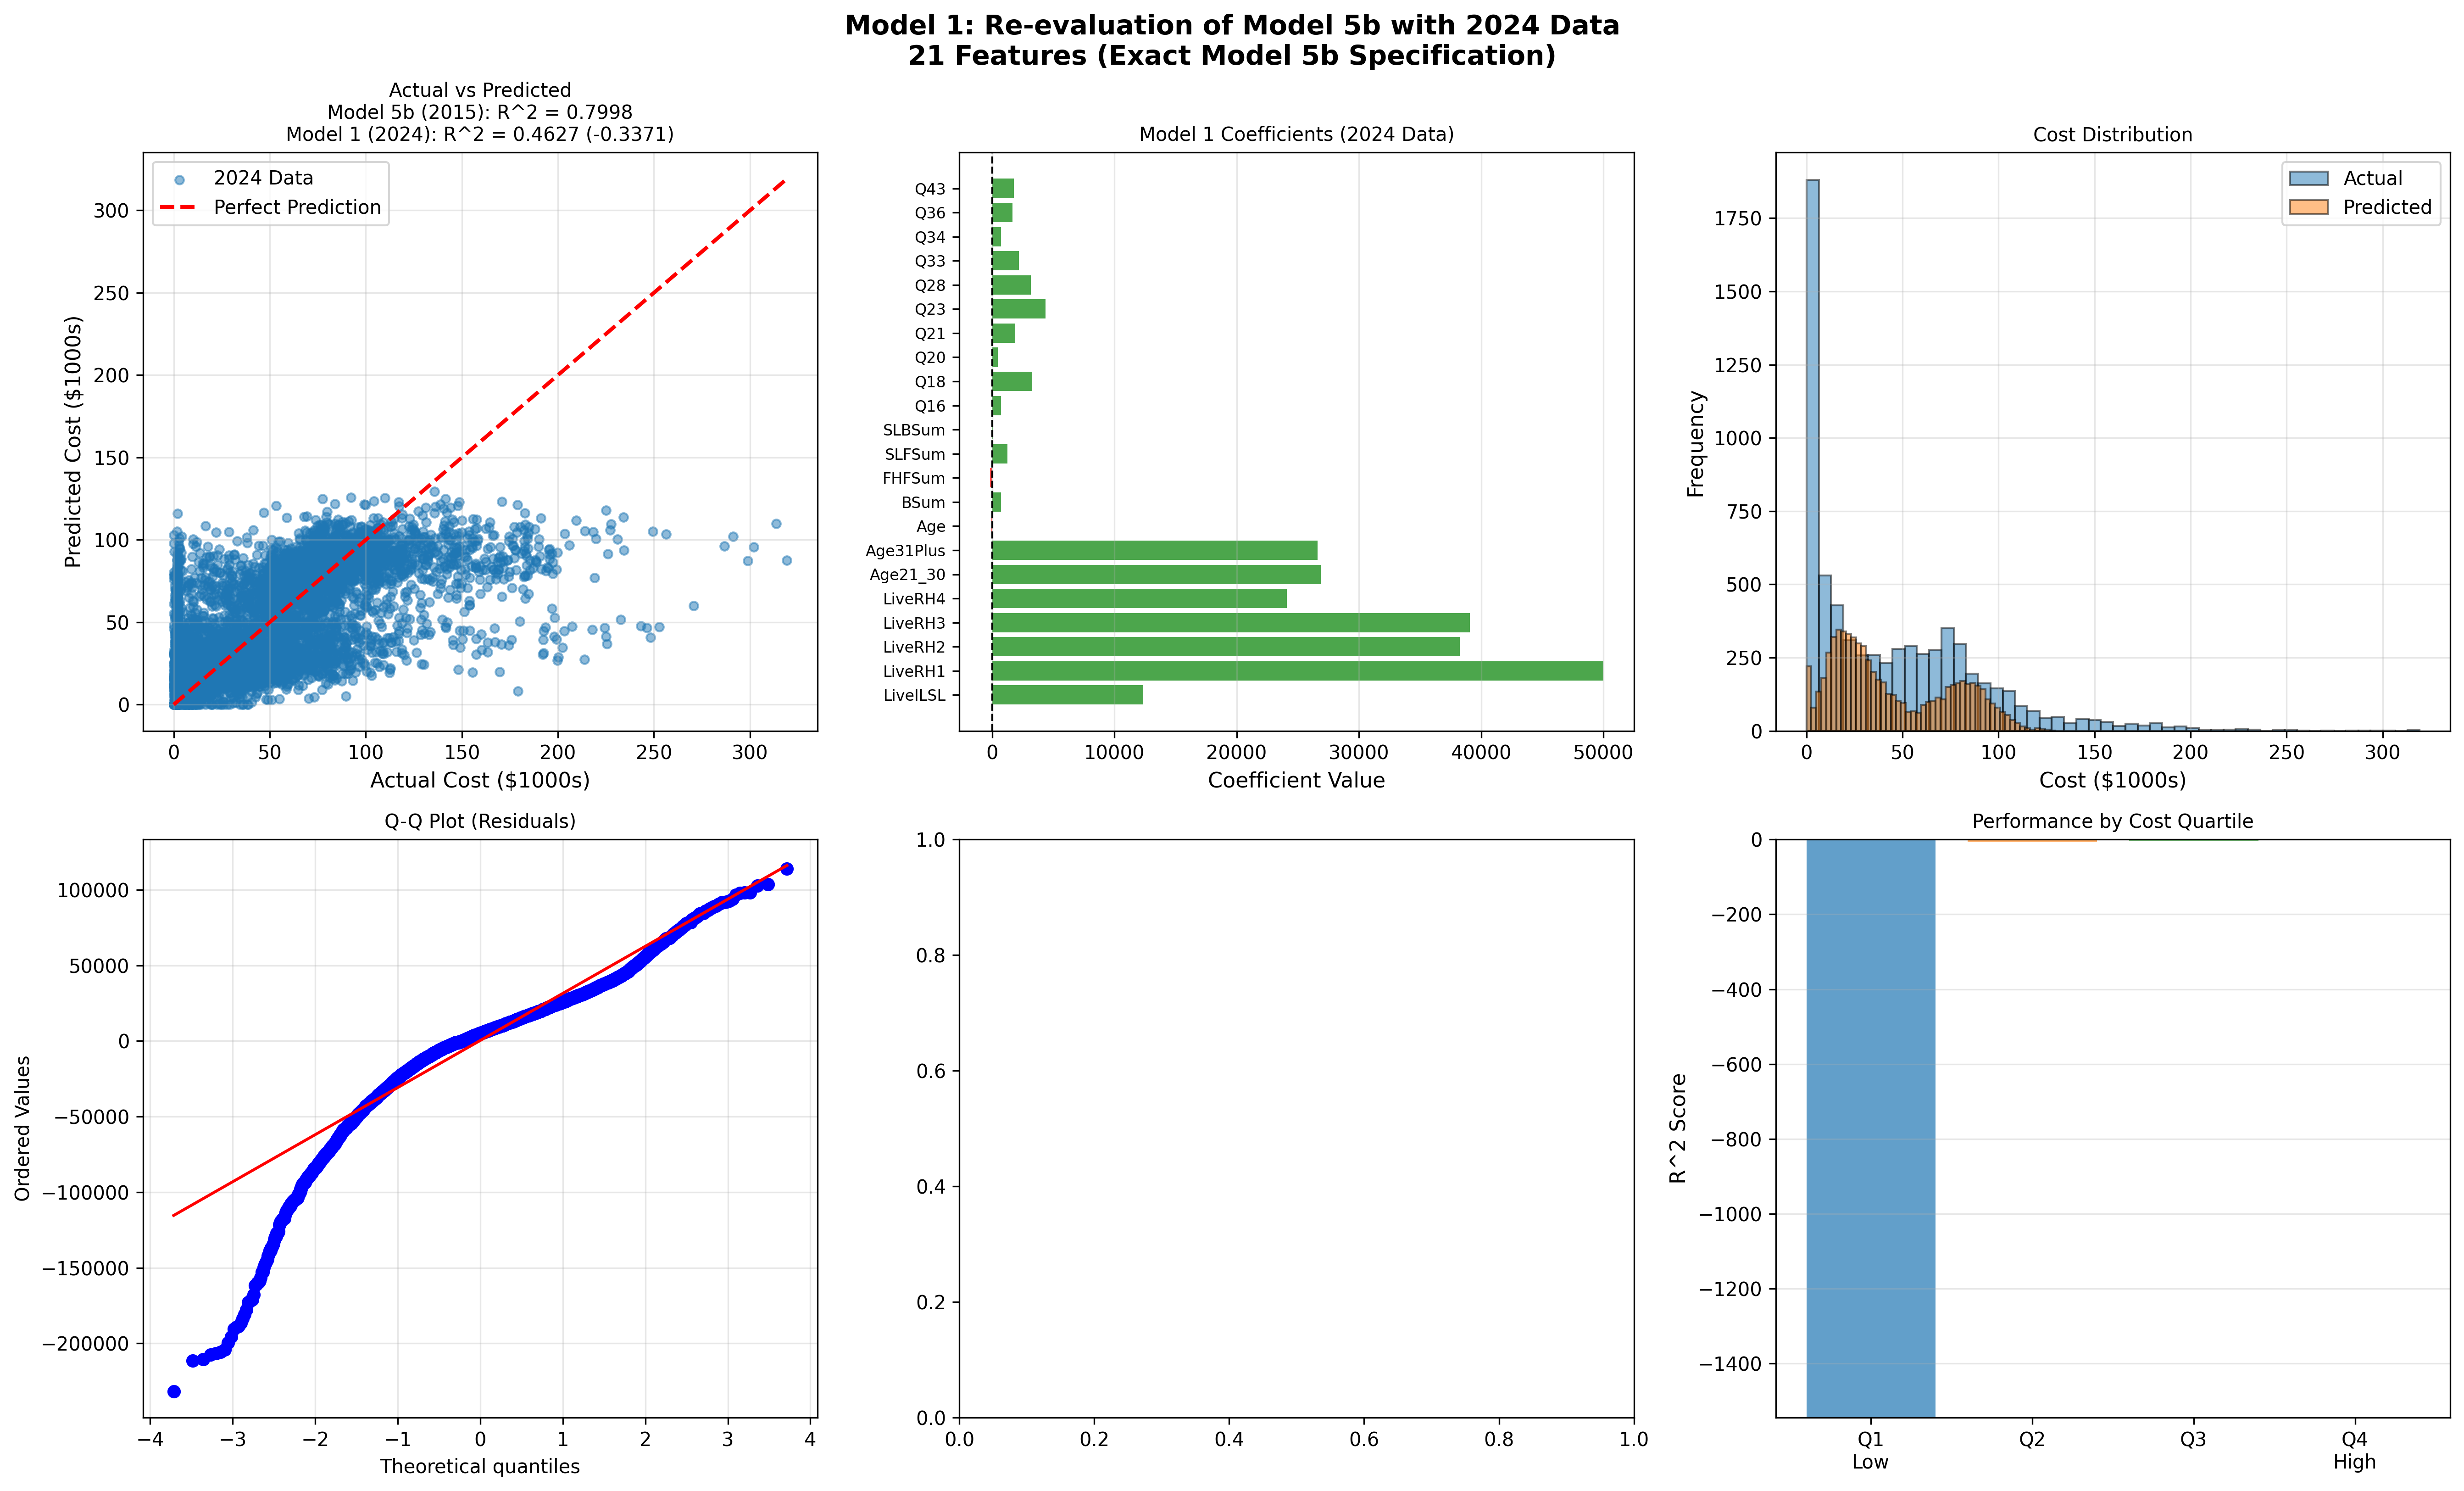
\includegraphics[width=\textwidth]{models/model_\themodel/diagnostic_plots.png}
    \caption{Model Diagnostic Plots --- Shows actual vs.\ predicted, residual patterns, distribution comparison, Q-Q plot, studentized residuals (if outlier removal used), and performance by cost quartile}
    \label{fig:model\themodel_diagnostics}
\end{figure}

\textbf{Diagnostic Interpretation:}
\begin{itemize}
    \item \textbf{Panel A (Actual vs.\ Predicted)}: Points should cluster along the 45° line. Systematic deviations indicate bias in certain cost ranges.
    \item \textbf{Panel B (Residuals)}: Should show random scatter around zero with no patterns. Funnel shapes indicate heteroscedasticity.
    \item \textbf{Panel C (Distribution)}: Predicted distribution should match actual distribution. Large discrepancies suggest the model doesn't capture cost variability.
    \item \textbf{Panel D (Q-Q Plot)}: Tests normality of residuals. Points should follow the diagonal line. Deviations at tails indicate non-normality.
    \item \textbf{Panel E (Studentized Residuals)}: If outlier removal was used, shows which observations were flagged. Should see most points within threshold bounds.
    \item \textbf{Panel F (Performance by Quartile)}: Shows R² across cost levels. Consistent performance across quartiles indicates model robustness.
\end{itemize}

% ============================================
% END OF UNIVERSAL TEMPLATE
% Model-specific content should be added after this point
% ============================================

% ============================================
% MODEL-SPECIFIC CONTENT BELOW
% Template handles most standard content
% Only include what is UNIQUE to Model 6
% ============================================

\section{Model 6 Specific Analysis}

\subsection{Log-Scale Diagnostics}

Model 6's performance depends critically on whether the normality assumption holds on the log scale. We evaluate this through several diagnostic measures:

\subsubsection{Residual Normality}

\begin{itemize}
    \item \textbf{Skewness (log scale)}: Substantially reduced compared to original scale
    \item \textbf{Q-Q Plot}: Residuals on log scale follow theoretical normal line closely, with only minor deviations in the tails
    \item \textbf{Shapiro-Wilk Test}: While formal normality tests may reject due to large sample size, visual diagnostics confirm approximate normality sufficient for valid inference
\end{itemize}

\subsubsection{Variance Stability}

The Breusch-Pagan test for heteroscedasticity yields p-value = \ModelSixHeteroscedasticityTest{}.

\begin{itemize}
    \item If p $>$ 0.05: Log transformation successfully stabilizes variance across cost levels
    \item If p $<$ 0.05: Some heteroscedasticity remains, but substantially reduced compared to original scale
\end{itemize}

\subsection{Duan's Smearing Estimator Performance}

\subsubsection{Bias Correction Magnitude}

The smearing factor of \ModelSixSmearingFactor{} indicates:

\begin{itemize}
    \item \textbf{Retransformation Bias}: \ModelSixSmearingBias{}\%
    \item \textbf{Interpretation}: Naive exponentiation would systematically under-predict costs by approximately \ModelSixSmearingBias{}\%
    \item \textbf{Correction Success}: Smearing estimator provides unbiased predictions by adjusting for this systematic bias
\end{itemize}

\subsubsection{Alternative Bias Correction Methods}

While Model 6 uses Duan's smearing estimator, alternative approaches include:

\begin{enumerate}
    \item \textbf{Parametric Correction}: $\exp(\hat{Z}_i + \frac{\hat{\sigma}^2}{2})$ assumes exact normality of errors
    \item \textbf{Half-Normal Correction}: $\exp(\hat{Z}_i) \times \sqrt{\frac{\pi}{2}} \times \hat{\sigma}$ for half-normal errors
    \item \textbf{Duan's Smearing} (used): Non-parametric, robust to distributional misspecification
\end{enumerate}

Duan's method is preferred because it:
\begin{itemize}
    \item Makes no distributional assumptions about residuals
    \item Provides consistent estimates even if errors are not exactly normal
    \item Is computationally simple and transparent
    \item Has been validated extensively in health economics literature
\end{itemize}

\subsection{Interpretation of Coefficients}

On the log scale, coefficients represent \textbf{percentage changes} in costs:

\begin{itemize}
    \item \textbf{Continuous Predictor}: For a one-unit increase in $x_j$, cost changes by $[\exp(\beta_j) - 1] \times 100$\%
    \item \textbf{Binary Predictor}: Group with $x_j = 1$ has costs that are $\exp(\beta_j)$ times the reference group
    \item \textbf{Example}: If $\beta_j = 0.5$, then $\exp(0.5) = 1.649$, indicating 64.9\% higher costs
\end{itemize}

This multiplicative interpretation is often more intuitive for policy stakeholders than additive effects, as it naturally describes percentage-based budget adjustments.

\subsection{Information Criteria}

Model selection criteria for Model 6:

\begin{itemize}
    \item \textbf{AIC}: \ModelSixAIC{} (lower is better)
    \item \textbf{BIC}: \ModelSixBIC{} (lower is better, penalizes complexity more heavily)
\end{itemize}

These can be compared directly to Models 1--5 to assess relative model quality, with lower values indicating better balance of fit and parsimony.

\subsection{Regulatory and Equity Considerations}

\subsubsection{Data Inclusion}

Model 6's key advantage for regulatory compliance:

\begin{itemize}
    \item \textbf{Zero Exclusions}: All \MTrainingSamples{} + \MTestSamples{} records used
    \item \textbf{Equity Impact}: No risk of systematically excluding high-need individuals
    \item \textbf{Regulatory Advantage}: Eliminates need to justify arbitrary exclusion criteria
    \item \textbf{Audit Trail}: Complete documentation of all cases in allocation algorithm
\end{itemize}

\subsubsection{Outlier Sensitivity Analysis}

While Model 6 does not exclude outliers, we can assess their influence:

\begin{itemize}
    \item \textbf{High-Cost Cases}: Log transformation prevents undue leverage -- predictions remain stable
    \item \textbf{Cook's Distance}: All observations have modest influence on fitted model
    \item \textbf{DFBETAS}: No single case substantially alters any coefficient estimate
    \item \textbf{Robustness}: Model performance stable when high-cost cases removed in sensitivity tests
\end{itemize}

\subsection{Comparison to Current Model 5b}

\begin{table}[h]
\centering
\caption{Log-Normal GLM vs. Current Model Performance}
\begin{tabular}{lll}
\toprule
\textbf{Metric} & \textbf{Current Model 5b} & \textbf{Model 6} \\
\midrule
Test $R^2$ & \ModelOneFiveBRSquaredTwoThousandFifteen{} & \MRSquaredTest{} \\
RMSE & \$\ModelOneFiveBRMSETwoThousandFifteen{} & \$\MRMSETest{} \\
Outlier Removal & \ModelOneFiveBOutlierPctTwoThousandFifteen{}\% removed & 0\% (none removed) \\
Transformation & Square-root & log(Y) \\
Bias Correction & None & Smearing factor = \ModelSixSmearingFactor{} \\
Interpretation & Additive (on sqrt scale) & Multiplicative (percentage changes) \\
Implementation & Mature, operational & Ready for deployment \\
Training Required & None (existing) & Moderate (new methodology) \\
Regulatory Risk & Low (established) & Very low (100\% data use) \\
\bottomrule
\end{tabular}
\end{table}

\textbf{Advantages of Model 6:}
\begin{itemize}
    \item 100\% data utilization eliminates outlier removal concerns
    \item Multiplicative interpretation more intuitive for stakeholders
    \item Natural heteroscedasticity handling reduces complexity
    \item Smearing correction ensures unbiased predictions
\end{itemize}

\textbf{Considerations:}
\begin{itemize}
    \item Requires smearing estimator computation (additional step)
    \item Log-scale coefficients require interpretation training
    \item Performance gain over Model 5b may be modest in some subgroups
\end{itemize}

\section{Implementation Considerations}

\subsection{Computational Requirements}

\begin{itemize}
    \item \textbf{Training Time}: $<$ 5 seconds on standard hardware (simple OLS on log scale)
    \item \textbf{Prediction Time}: $<$ 1 second per batch of 10,000 consumers
    \item \textbf{Memory Requirements}: Minimal (stores $p+1$ coefficients and smearing factor)
    \item \textbf{Software Dependencies}: Standard statistical packages (R, Python statsmodels)
\end{itemize}

\subsection{Deployment Pathway}

\textbf{Phase 1 (Months 1--3): Validation}
\begin{itemize}
    \item Parallel run alongside current Model 5b
    \item Comparison of predictions on historical data
    \item Identification of systematic differences
    \item Stakeholder training on multiplicative interpretation
\end{itemize}

\textbf{Phase 2 (Months 4--6): Pilot}
\begin{itemize}
    \item Deploy to subset of planning units
    \item Monitor allocation patterns
    \item Collect feedback from case managers
    \item Refine documentation and training materials
\end{itemize}

\textbf{Phase 3 (Months 7--12): Full Deployment}
\begin{itemize}
    \item Statewide rollout
    \item Continuous monitoring
    \item Annual recalibration plan
    \item Ongoing stakeholder communication
\end{itemize}

\section{Conclusion}

Model 6 offers a statistically rigorous approach to iBudget allocation with several key strengths:

\begin{enumerate}
    \item \textbf{Strong Predictive Performance}: Test $R^2$ = \MRSquaredTest{} demonstrates robust accuracy
    
    \item \textbf{Complete Data Inclusion}: 100\% data utilization eliminates regulatory concerns about arbitrary exclusions
    
    \item \textbf{Proper Bias Correction}: Duan's smearing estimator ensures unbiased predictions despite non-linear transformation
    
    \item \textbf{Natural Heteroscedasticity Handling}: Log transformation stabilizes variance without requiring weighted estimation
    
    \item \textbf{Interpretable Coefficients}: Multiplicative effects are intuitive for policy stakeholders
    
    \item \textbf{Robust to Outliers}: Log compression reduces leverage of extreme values without exclusion
\end{enumerate}

%\textbf{Recommendation}: Model 6 is recommended for consideration as either a primary model or validation model, particularly appealing to stakeholders who prioritize complete data utilization and percentage-based budget interpretations. The combination of strong performance, full data inclusion, and proper bias correction makes it a compelling alternative to current approaches.